\chapter{Anatomy \& Function}
\label{chap: anatomy}

\section{Introduction}

The mammalian central nervous system is often divided into the brain stem, limbic system, cerebellum, and cerebrum. The brain stem, which sits at the base, is composed of the medulla, pons, and mid-brain. It plays a role in regulating basic biological functions, such as heart rate, breathing, eating, sleeping, etc. The limbic system is a collection of structures that sit on top of the brain stem. These structures consist of the hippocampal formation, hypothalamus, thalamus, and amygdala. The cerebellum sits behind the other areas, and is a dense, highly folded sheet of neurons that is often associated with posture and movement. The cerebrum contains the cerebral cortex, another highly folded sheet of neurons, consisting of four lobes that sit on top of the limbic system. It is associated with a variety of ``higher order" cognitive capacities, such as sensory processing, memory, language, movement, planning, etc. The cerebrum also contains a variety of sub-cortical structures, such as the basal ganglia and olfactory bulb.


\section{Brain Stem}

\subsection{Midbrain}

\subsection{Pons}

\subsection{Medulla Oblongata}


\section{Limbic System}

Limbic system is shown in Figure \ref{fig: limbic system}.

\begin{figure}[h]
    \centering
    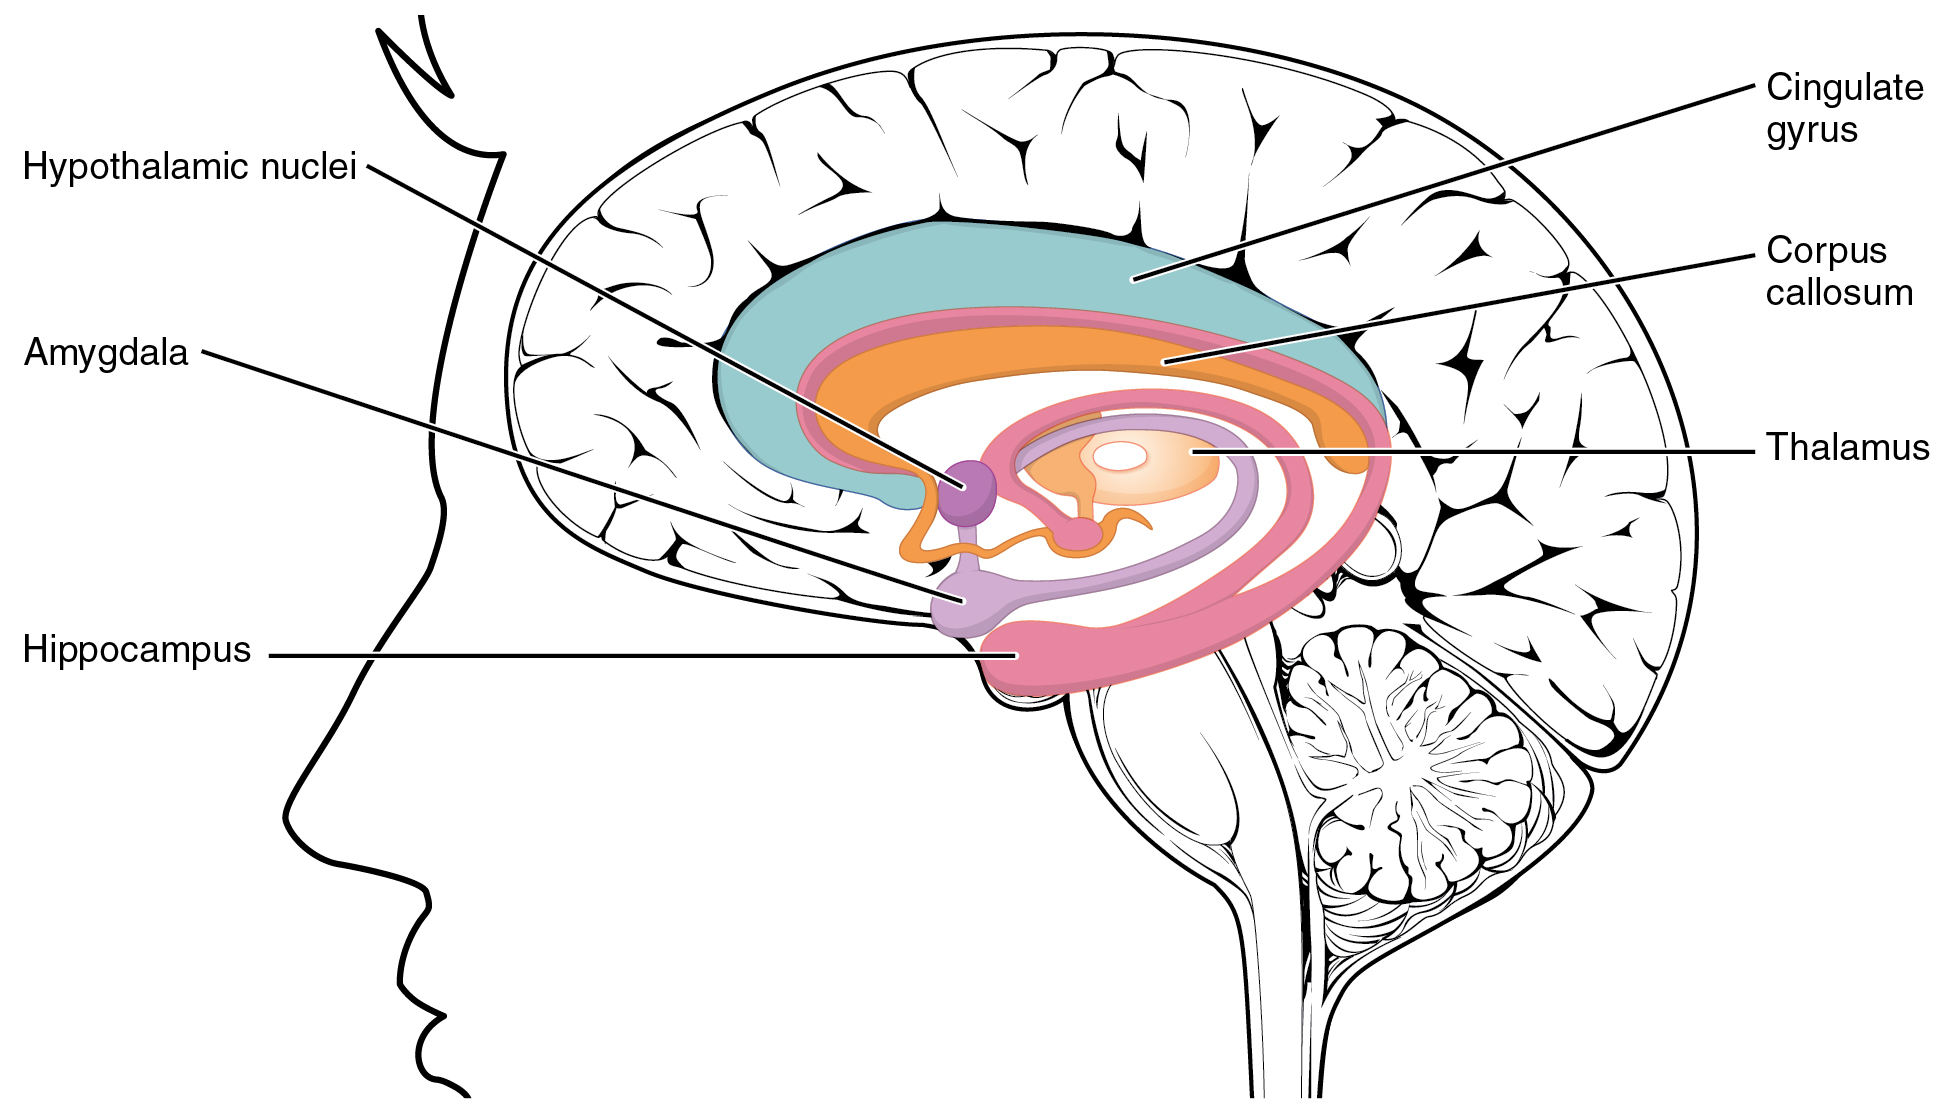
\includegraphics[width=.75\textwidth]{images/neuroscience/limbic_system.jpg}
    \caption{The limbic system. From https://cnx.org/.}
    \label{fig: limbic system}
\end{figure}



\subsection{Thalamus}


\subsection{Hippocampus}

The hippocampus is a bilateral structure located in the medial temporal lobes. It is a component of the hippocampal formation, which is comprised of the hippocampus itself, along with the dentate gyrus and the subiculum. At times, other structures, such as entorhinal cortex, are included in the hippocampal formation.


\subsubsection{Memory Consolidation}

The hippocampus plays a role in memory consolidation, acting to initially encode memories (``one-shot" encoding), which are later consolidated in cortex. This cooperative aspect between hippocampus and cortex is the main idea put forward by the complementary learning systems (CLS) theory \cite{mcclelland1995there, kumaran2016learning}. Early evidence for this hypothesis came from the human subject H.M., who experienced a gradient of retrograde amnesia following the surgical removal of his medial temporal lobes \cite{penfield1958memory}. H.M. could recall memories from childhood, however, events in the recent past could not be easily recalled. Further evidence has helped to support this hypothesis, in addition to adding further nuance. Hippocampal ``replay" is a phenomenon that occurs during sleeping or restful states, whereby recent neural activity is replayed, typically at a faster speed. There is evidence to suggest that this replay mechanism is important for retaining information \cite{girardeau2009selective}, though this evidence is not conclusive. There is also evidence that replay occurs more frequently for novel, salient experiences \cite{foster2006reverse, singer2009rewarded}. This memory consolidation functionality has been adopted in the reinforcement learning community in the form of ``replay buffers," which collect recent trajectories of experiences to later use for training \cite{mnih2013playing}. These replay buffers appear to be essential for effectively training deep networks to perform a range of simulated tasks, helping to stabilize training. Interestingly, re-weighting replay according to the temporal difference error, a measure of reward novelty, yields further improved results \cite{schaul2015prioritized}.


\subsubsection{Spatial Memory \& Navigation}

The hippocampus is involved in spatial memory and navigation. Striking evidence for this is the presence of place cells, pyramidal neurons in CA1 and CA3 that fire when the animal is in particular spatial locations, known as place fields. 


\subsubsection{Planning}

Hippocampus also assists in planning. While it is difficult to precisely assess, there is evidence to suggest that hippocampal replay can be used ``online" during tasks to plan future trajectories \cite{o2010play, olafsdottir2018role}. Likewise, other memories appear to be replayed during online behavior, perhaps encoding other prior, task-relevant information. Some of this replay may also just be part of memory consolidation. There is also evidence that selective impairment of hippocampus results in performance deficits in multi-step model-based planning \cite{miller2017dorsal}. In addition to amnesia \cite{barash2018acute}, reports in humans with abnormal hippocampal activity induced through drug overdoses also report deficits in planning capabilities.


\subsection{Olfactory Bulb}

\subsection{Hypothalamus}

\subsection{Amygdala}



\section{Cerebrum}

\subsection{Basal Ganglia}

The basal ganglia play a role in dopamine release. From Josh Berke: The dynamically changing dopamine signal corresponds well to a value function. This value function provides an estimate of available (temporally discounted) reward that influences decisions to work. Abrupt changes in this signal are used as a reward prediction error (RPE), which can be used to reinforce choice behavior. The dopamine cells in the midbrain (basal ganglia) project to the forebrain. However, these forebrain dopamine cells are not simply a passive read-out of midbrain cell activity. Dopamine appears to be useful for both real-time motivation as well a reward-based learning.

\subsubsection{Striatum}

In reinforcement learning terms, the (dorsolateral) striatum is associated with model-free, value-based learning \cite{daw2005uncertainty}.

\subsubsection{Substantia Nigra}

\subsubsection{Pallidum}

\subsubsection{Subthalamic Nucleus}


\subsection{Cerebral Cortex}





\section{Cerebellum}